\documentclass{article}
\usepackage{graphicx}
\usepackage{spverbatim}
\begin{document}
\title{Kuwahara Filter}
\date{Nov 2024}

\section{Implement the Labwork}
\subsection{Kuwahara Filter}
The Kuwahara filter is a non-linear smoothing filter used in image processing for adaptive noise reduction.

The steps to implement the Kuwahara filter are as follows:
\begin{itemize}
    \item Convert the image from RGB to HSV color space.
    \item Divide the image into 4 overlapping blocks, provided windows size (W), the size of each block is (W//2 + 1).
    \item For each block, calculate the variance of the V value in HSV colorspace in the block.
    \item Find the minimum variance value and its corresponding block, choose this block as the filter window.
    \item Replace the pixel value in the center of the block with the average value of the pixels in the choosen block.
\end{itemize}

Next we will go through the implementation of the Kuwahara filter on GPU.

My strategy is each thread will process one pixel in the image, including visiting 4 subregions corresponding with the pixel, the calculation of the variance and the replacement of the pixel value.
\begin{itemize}
    \item First of all, I reused the HSV convert function from the previous labwork. This HSV labwork very helpful, it convert RGB from Array of Struct to Struct of Array, which is more sufficient because we only need the V channel in this labwork.
    \item Next, I implemented the kernel function to divide each windows into 4 subregions, calculate the variance of the V value in each subregion, and find the minimum variance value, replace the pixel value in the center of the block with the average value of the pixels in the choosen block.
\end{itemize}

The process looks like this:
\begin{spverbatim}
    # Find the sub_regions with min variance
    min_variances = np.inf
    best_leftx, best_topy = 0, 0
    for iy in [-offset, 0]:
        for ix in [-offset, 0]:
            left_x = max(0, tidx+ix)
            top_y = max(0, tidy+iy)
            variances = variance_of(d_v_input, left_x, top_y, offset, img_h, img_w)
            if variances < min_variances:
                min_variances = variances
                best_leftx, best_topy = left_x, top_y
    # Calculate the mean (r, g, b) of best variance
    r, g, b = mean_rgb_of(
        d_image,
        best_leftx, 
        best_topy, 
        offset, 
        img_h, img_w
    )
    
    d_output[tidy, tidx, 0] = r
    d_output[tidy, tidx, 1] = g
    d_output[tidy, tidx, 2] = b
\end{spverbatim}
\subsection{Kuwahara Filter with CPU}
I also implemented the Kuwahara filter on CPU for comparison. For simplicity, I used rgb\_to\_hsv function of matplotlib package to convert RGB to HSV color space, then the rest of the process is the same as the GPU implementation.

\section{Experiment}
Since Google Colab is unstable for benchmarking, I've run the experiment on a VastAI server with the following specifications:
\begin{itemize}
    \item 1 x RTX 3060
    \item Xeon® E5-2699 v3
\end{itemize}
Because Numba need the first run to compile the code, I run the experiment with 5 runs and only capture the time of the last one.
\begin{spverbatim}
# run multiple time and get the last one as the runtime
for i in range(5):
    start_t = time.time()
    rgb2hsv[gridSize, block_size](d_input, d_hsv_output, img_h, img_w)
    d_v_input = d_hsv_output[2]
    kernel[gridSize, block_size](d_input, d_v_input, d_output, window_size, img_h, img_w)
    cuda.synchronize()
    dst = d_output.copy_to_host()

ct = time.time() - start_t
\end{spverbatim}

\subsection{Experiment with different block size values}
I've experimented with block size values of [(8, 8), (16, 16), (32, 32)]. We only experiment at max 32x32 block size since the max thread per block is 1024, and the block size is limited by the number of threads per block.
The result is as follows:
\begin{figure}
    \centering
    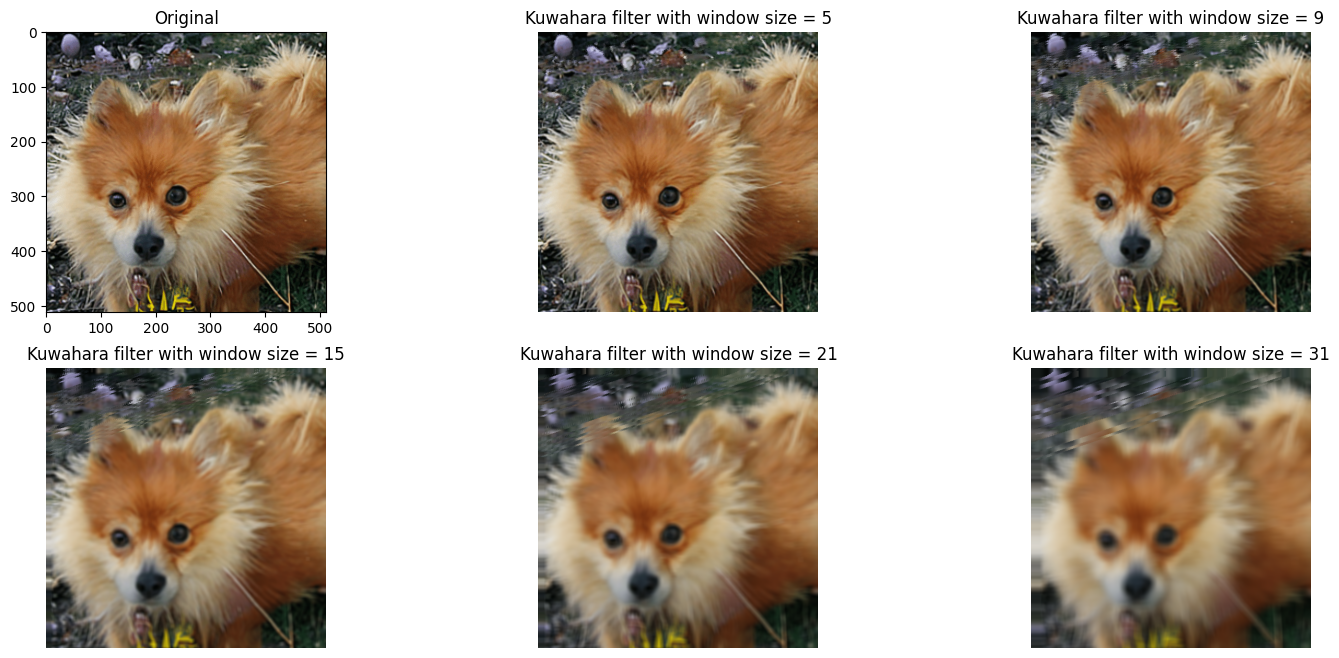
\includegraphics[width=0.5\linewidth]{results/output.png}
    \caption{Kuwahara Filter with various block size values}
    \label{fig:enter-label}
\end{figure}
\begin{figure}
  \centering
  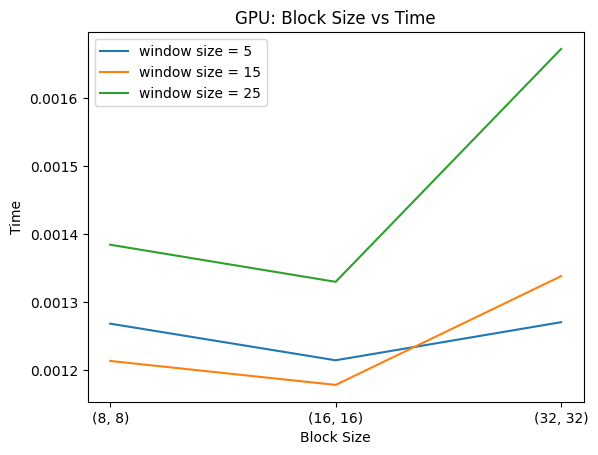
\includegraphics[width=0.5\linewidth]{results/gpu_blocksize_vs_time.png}
  \caption{Kuwahara Filter runtime with various block size values}
  \label{fig:enter-label}
\end{figure}
The chart shows the best block size value is (16, 16) in different image dimensions.

\subsection{Speedup GPU vs CPU}
In this experiment, I will visualize the speedup of the GPU implementation compared to the CPU implementation with configuration of block size (16, 16) in various image dimensions. I prepared one image, then took the 20\%, 40\%, 60\%, 80\% and 100\% of the image to experiment. The result is as follows:
\begin{figure}
  \centering
  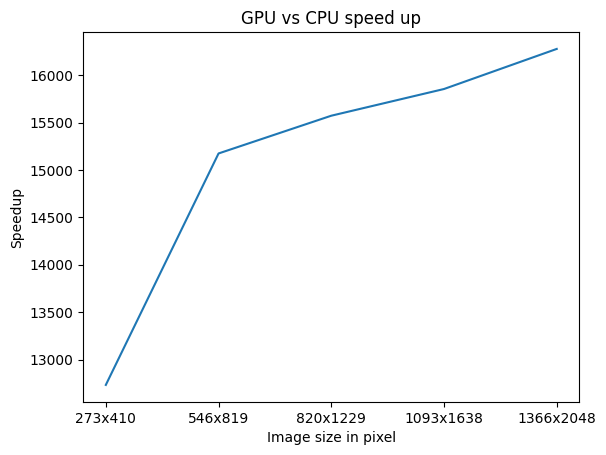
\includegraphics[width=0.5\linewidth]{results/speedup.png}
  \caption{GPU vs CPU speedup}
  \label{fig:enter-label}
\end{figure}
The chart shows the speedup of the GPU implementation compared to the CPU implementation is significant, especially in large image dimensions.

Looking at the chart, the speed-up (ratio of GPU time to CPU time) increases significantly with the image size. This suggests that the GPU handles larger images much more efficiently than the CPU.

While the speed-up is increasing, the rate of increase seems to slow down slightly with each increment. This could indicate that as the image size grows beyond a certain point, the GPU's shared memory or memory bandwidth might start to become a limiting factor.

\section{Future Improvement}
There is an idea to improve the Kuwahara filter by using the shared memory to store the V value of the block, which can reduce the memory access time and improve the performance of the filter. We can store the V value of the block in the shared memory, then calculate the variance and the mean of the block in the shared memory.
The maximum shared memory per block is 48KB, so we can store the V value of the block (4 bytes) with a size of 16x16, even with 32x32.

\end{document}